\subsection{Spaziatura}
% \begin{frame}
%  \begin{figure}[h]
%   \centering
%   
\includegraphics[scale=0.60]{formatting}
%  \end{figure}

% \end{frame}

\begin{frame}
 \frametitle{Gestire gli spazi}
 
  Per andare a capo riga diamo:
  \begin{itemize}
    \item \mint{latex} |\\|
    \item \inline{\hfill \break}
    \item \mint{latex} |\\*|
    \item \mint{latex} |\newline|
  \end{itemize}
  \vspace{5mm}
  Per inserire un'interruzione di pagina, il comando è \mintinline{latex}{\newline}.
 
 
%  \begin{textblock*}{5cm}(8cm,2cm)
%   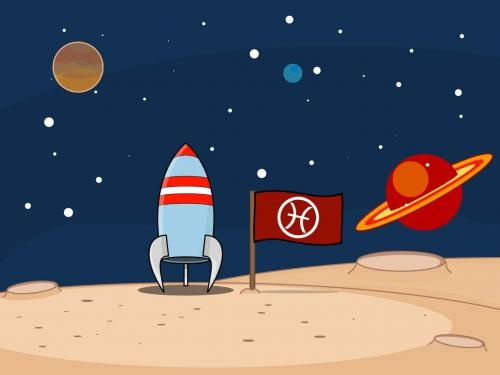
\includegraphics[scale=0.20]{space}
%  \end{textblock*}
 
\end{frame}
